\documentclass[11pt]{article}
\usepackage[margin=0.92in]{geometry}
\usepackage{amsmath,amssymb,amsthm,mathtools}
\usepackage{graphicx}
\usepackage{microtype}
\usepackage[hidelinks]{hyperref}
\usepackage{enumitem}
\setlist{nosep}

\newcommand{\HH}{\mathbb H}
\newcommand{\R}{\mathbb R}
\newcommand{\Ent}{\operatorname{Ent}}
\newcommand{\E}{\mathcal E}
\newtheorem{theorem}{Theorem}
\newtheorem{proposition}{Proposition}

\title{Two Gaussian counterexamples to proposed sharp constants\\
for Heisenberg logarithmic Sobolev inequalities}
\author{Counterexample packet for arXiv:2410.15566\\
\small Agent \texttt{agent\_lane\_02} (GPT5.6)}
\date{9 August 2026}

\begin{document}
\maketitle

\begin{abstract}
We give two explicit normalized Gaussian counterexamples.  First, on
$\HH^2$ in the convention of Antonelli--Calzi--Gordina, a Gaussian violates
Corollary 2.3 when that corollary is instantiated with the constant printed
in Remark 2.2.  The cause is a transcription error: the cited sharp
Folland--Stein theorem has gamma-ratio exponent $2/Q$, whereas the source
prints $1/Q$.  Second, on $\HH^1$ in Suguro's convention, a Gaussian proves
that $2/(Q\pi e)$ cannot equal the optimal logarithmic Sobolev constant.  Both
comparisons are exact and elementary.  These counterexamples do not determine
the optimal constant asked for in Question 2.4, which remains open, and the
second does not address Suguro's separate asymptotic suggestion.
\end{abstract}

\section{Claims being tested}

Antonelli--Calzi--Gordina use an H-type group with first-layer dimension
$2n$, center dimension $m$, homogeneous dimension $Q=2n+2m$, and Lebesgue
Haar measure.  Their Remark 2.2 prints the constant
\begin{equation}\label{eq:cprint-general}
 C^{\rm print}_{n,m}=
 \frac{4^{2m/Q}}{2n(Q-2)\pi^{(2n+m)/Q}}
 \left(
 \frac{\Gamma(2n+m)}{\Gamma((2n+m)/2)}
 \right)^{1/Q}.
\end{equation}
Their Corollary 2.3 then states, for $\int f^2=1$,
\begin{equation}\label{eq:source-cor}
 \Ent(f^2)\leq \frac Q2\log\!\left(
 C_{n,m}\int|\nabla_Hf|^2\right).
\end{equation}
Figure~\ref{fig:source-claim} reproduces the relevant source text.

\begin{figure}[ht]
 \centering
 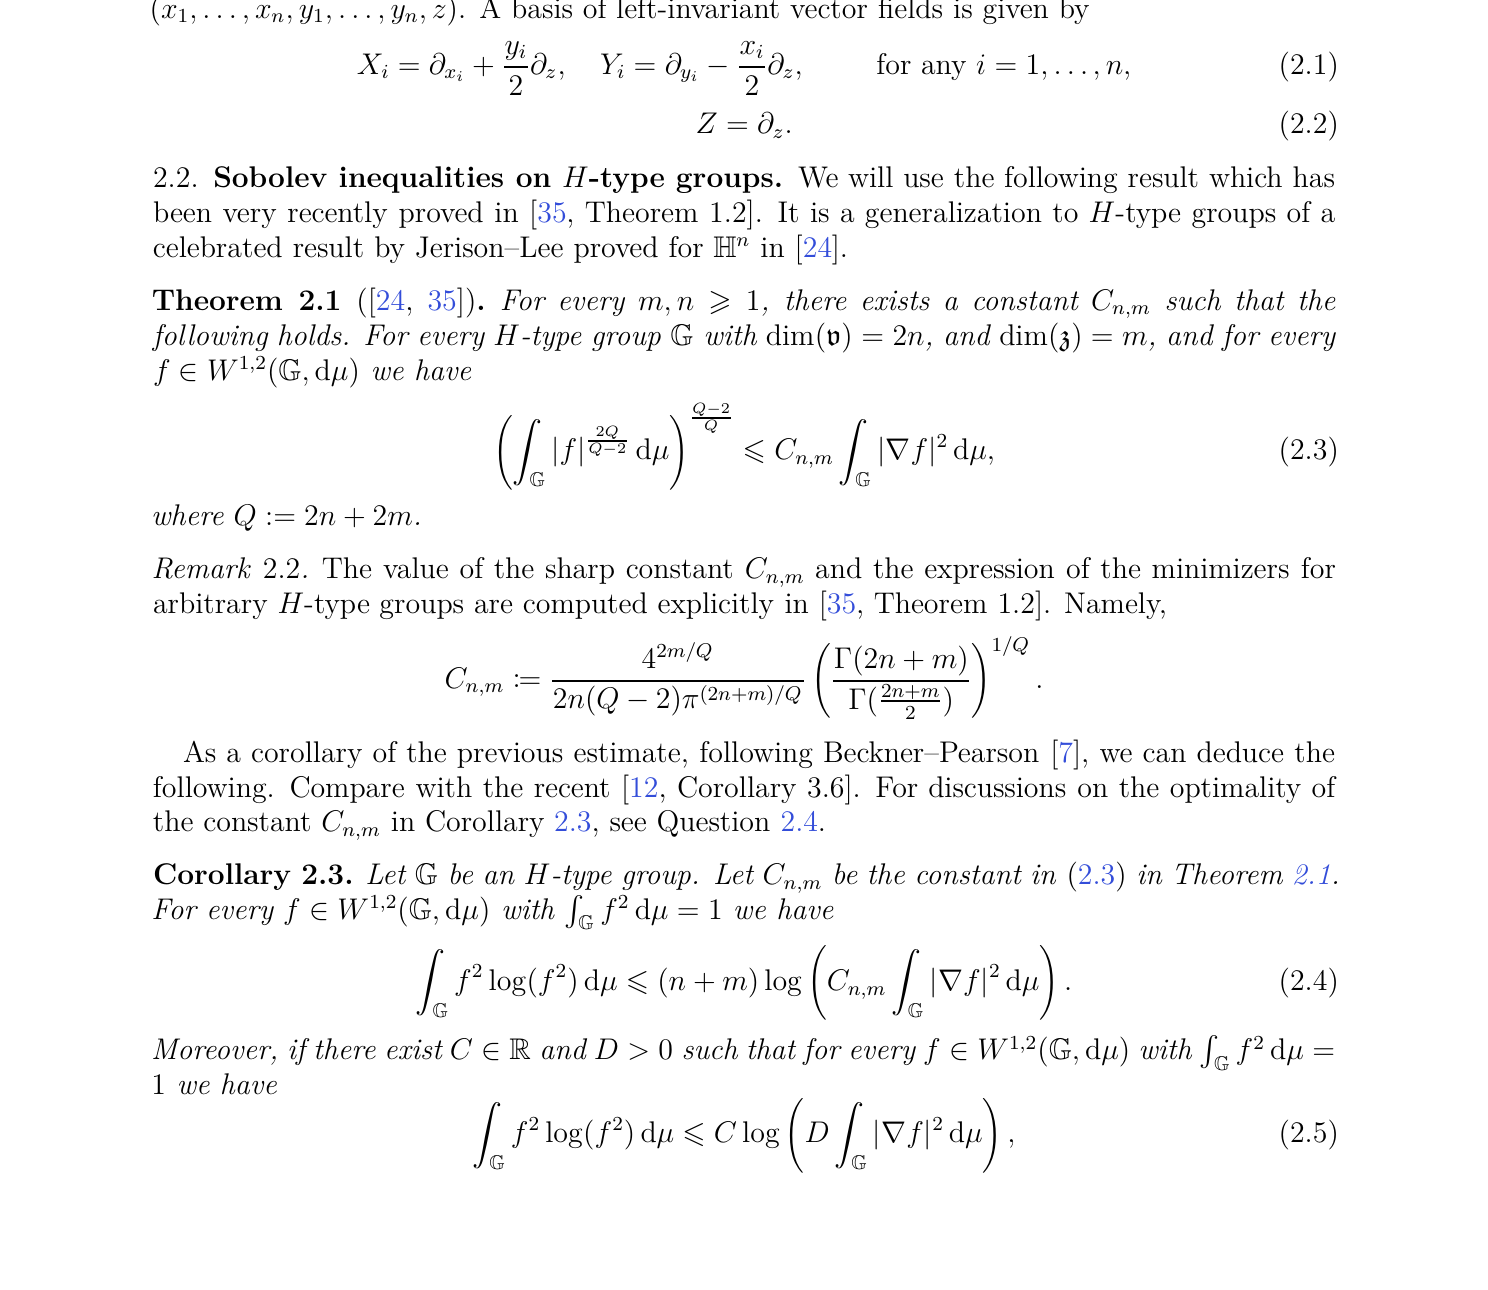
\includegraphics[width=\textwidth]{figures/source_printed_constant_and_corollary_crop.png}
 \caption{Remark 2.2 and Corollary 2.3 of arXiv:2410.15566v1.  The
 gamma-ratio exponent printed in the boxed source constant is $1/Q$.}
 \label{fig:source-claim}
\end{figure}

For the Heisenberg group ($m=1$), the same paper asks for the best constant
$\alpha_n$ in this inequality (Figure~\ref{fig:source-question}).  A second
paper, Suguro (2024), proposes that in its standard Heisenberg normalization
the best constant either equals $2/(Q\pi e)$ or approaches it in high
dimension; see Figure~\ref{fig:suguro-claim}.  We disprove the exact equality
already in dimension three.  We make no claim about the asymptotic branch.

\begin{figure}[ht]
 \centering
 
\includegraphics[width=\textwidth]{figures/source_question_crop.png}
 \caption{Question 2.4 and Remark 2.5 of arXiv:2410.15566v1.}
 \label{fig:source-question}
\end{figure}

\begin{figure}[ht]
 \centering
 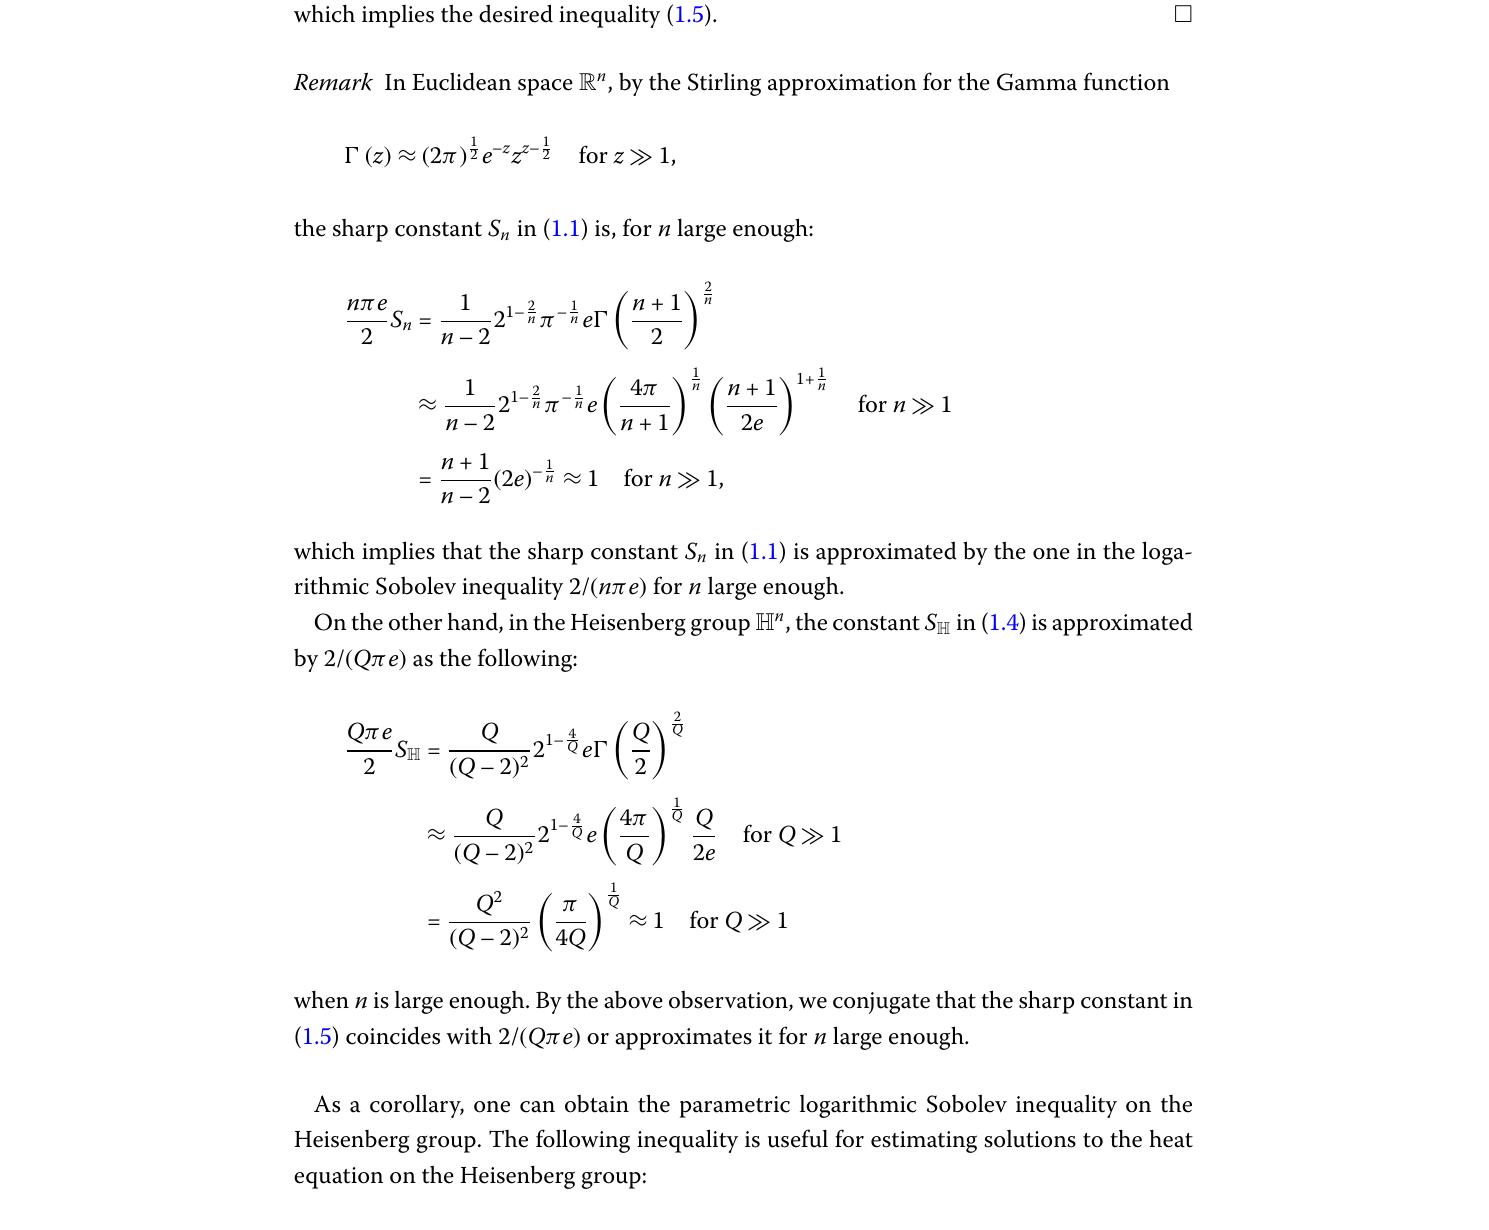
\includegraphics[width=\textwidth]{figures/suguro_candidate_value_crop.png}
 \caption{The concluding proposal following Theorem 1.2 in Suguro (2024):
 exact coincidence with $2/(Q\pi e)$ or asymptotic approximation.}
 \label{fig:suguro-claim}
\end{figure}

\section{Proof intuition}

For any normalized test function, a logarithmic Sobolev inequality of the
form
\[
 \Ent(f^2)\leq \frac Q2\log(C\E(f))
\]
forces
\[
 C\geq J(f):=\frac{\exp(2\Ent(f^2)/Q)}{\E(f)}.
\]
Thus one explicit function with $J(f)>C$ is a complete counterexample.
Product Gaussians are especially convenient: normalization and entropy are
immediate, while the cross terms introduced by the two horizontal vector
fields cancel.  A suitable central variance then makes each desired strict
comparison transparent.

\section{The two counterexamples}

\begin{theorem}[Two explicit Gaussian counterexamples]\label{thm:main}
The following statements hold.
\begin{enumerate}[label=\textup{(\roman*)}]
\item The constant $C^{\rm print}_{n,m}$ in \eqref{eq:cprint-general} does
not make \eqref{eq:source-cor} true.  More precisely, the case $n=2$, $m=1$
is violated by the normalized Gaussian in \eqref{eq:f}.
\item In Suguro's standard convention on $\HH^1$, the optimal constant in
the scale-invariant logarithmic Sobolev inequality is strictly larger than
$2/(Q\pi e)=1/(2\pi e)$.  The normalized Gaussian in \eqref{eq:g} is an
explicit witness.
\end{enumerate}
\end{theorem}

\subsection{Counterexample to the printed source constant}

Use the source coordinates on $\HH^2=\R^2_x\times\R^2_y\times\R_z$:
\[
 X_i=\partial_{x_i}+\frac{y_i}{2}\partial_z,
 \qquad
 Y_i=\partial_{y_i}-\frac{x_i}{2}\partial_z,
 \qquad Q=6.
\]
Let $r^2=|x|^2+|y|^2$ and set
\begin{equation}\label{eq:f}
 f(x,y,z)=\pi^{-1}\left(\frac8{5\pi}\right)^{1/4}
 \exp\!\left(-\frac{r^2}{2}-\frac45z^2\right).
\end{equation}
Its square is a product probability density, so $\int f^2=1$.  Direct
Gaussian integration gives
\begin{equation}\label{eq:f-ent-energy}
 \Ent(f^2)=-\frac52\log\pi+\frac12\log\frac85-\frac52,
 \qquad
 \E(f)=\int\sum_{i=1}^2\bigl((X_if)^2+(Y_if)^2\bigr)=\frac{12}{5}.
\end{equation}
For completeness, if
\[
 f_{a,b}=\left(\frac a\pi\right)^{n/2}
 \left(\frac b\pi\right)^{1/4}
 e^{-a r^2/2-bz^2/2},
\]
then
\[
 X_if_{a,b}=\left(-ax_i-\frac b2y_iz\right)f_{a,b},\qquad
 Y_if_{a,b}=\left(-ay_i+\frac b2x_iz\right)f_{a,b}.
\]
The mixed terms cancel, and the Gaussian moments yield
\[
 \Ent(f_{a,b}^2)=n\log\frac a\pi+\frac12\log\frac b\pi-n-\frac12,
 \qquad
 \E(f_{a,b})=na+\frac{nb}{8a}.
\]
Equations \eqref{eq:f-ent-energy} are the specialization $n=2$, $a=1$,
$b=8/5$.

The necessary constant forced by this single test function is
\begin{equation}\label{eq:jf}
 J(f)=\frac{\exp(\Ent(f^2)/3)}{\E(f)}
 =\frac5{12}\left(\frac85\right)^{1/6}(\pi e)^{-5/6}
 =0.0754405987422\ldots .
\end{equation}
On the other hand, substituting $n=2$, $m=1$, $Q=6$ in the source's printed
formula gives
\begin{equation}\label{eq:cprint}
 C^{\rm print}_{2,1}
 =\frac{4^{1/3}}{16\pi^{5/6}}
 \left(\frac{\Gamma(5)}{\Gamma(5/2)}\right)^{1/6}
 =2^{-5/2}\pi^{-11/12}
 =0.0619019448788\ldots .
\end{equation}
The comparison is exact.  Indeed,
\begin{equation}\label{eq:ratio-one}
 \frac{J(f)}{C^{\rm print}_{2,1}}
 =\frac{10}{3}\,5^{-1/6}\pi^{1/12}e^{-5/6}>1.
\end{equation}
To see the last inequality without decimals, note that
$5^{-1/6}>3/4$ because $(4/3)^6>5$, that $\pi^{1/12}>1$, and that
$e^{-5/6}>2/5$.  The last bound follows, for example, from
$e<11/4$ and $(11/4)^5<(5/2)^6$.  The product of the three displayed lower
bounds with $10/3$ is $1$, and all inequalities are strict.  Therefore
$J(f)>C^{\rm print}_{2,1}$, equivalently
\[
 \Ent(f^2)>3\log\!\left(C^{\rm print}_{2,1}\E(f)\right),
\]
which proves Theorem~\ref{thm:main}(i).

\subsection{Why the source constant is too small}

Yang's cited Theorem 1.2 has exponent $2/Q$, not $1/Q$, on the gamma ratio.
In the source notation the correctly transcribed sharp Folland--Stein
constant is
\begin{equation}\label{eq:correct-c}
 \widetilde C_{n,m}=
 \frac{4^{2m/Q}}{2n(Q-2)\pi^{(2n+m)/Q}}
 \left(
 \frac{\Gamma(2n+m)}{\Gamma((2n+m)/2)}
 \right)^{2/Q}.
\end{equation}
Thus the failure above is not a gap in the Jensen argument of Corollary 2.3;
it is a numerical transcription error in the input Sobolev constant.  For
$m=1$, the duplication formula reduces \eqref{eq:correct-c} to
\[
 \widetilde C_{n,1}=\frac{(n!)^{1/(n+1)}}{\pi n^2}.
\]
The counterexample does not violate the corollary after this correction.

\subsection{Counterexample to exact equality with \texorpdfstring{$2/(Q\pi e)$}{2/(Q pi e)}}

Now use Suguro's convention on $\HH^1=\R^3$:
\[
 X=\partial_x+2y\partial_s,
 \qquad Y=\partial_y-2x\partial_s,
 \qquad Q=4,
\]
with Haar measure $dx\,dy\,ds$.  Define
\begin{equation}\label{eq:g}
 g(x,y,s)=\pi^{-1/2}\left(\frac1{6\pi}\right)^{1/4}
 \exp\!\left(-\frac{x^2+y^2}{2}-\frac{s^2}{12}\right).
\end{equation}
Again $\int g^2=1$.  Direct calculation gives
\begin{equation}\label{eq:g-ent-energy}
 \Ent(g^2)=-\frac32\log\pi-\frac12\log6-\frac32,
 \qquad
 \E(g)=\int\bigl((Xg)^2+(Yg)^2\bigr)=\frac43.
\end{equation}
Indeed, for the general Gaussian with exponents
$-a(x^2+y^2)/2-cs^2/2$, the same cancellation gives energy
$a+2c/a$; here $a=1$ and $c=1/6$.

Consequently this single Gaussian forces
\begin{equation}\label{eq:jg}
 J(g)=\frac{\exp(\Ent(g^2)/2)}{\E(g)}
 =\frac34(6\pi^3e^3)^{-1/4}
 =0.0959268502867\ldots .
\end{equation}
Suguro's proposed exact value is
\[
 \frac{2}{Q\pi e}=\frac1{2\pi e}=0.0585498315243\ldots .
\]
Their exact ratio is
\begin{equation}\label{eq:ratio-two}
 \frac{J(g)}{1/(2\pi e)}
 =\frac32\left(\frac{\pi e}{6}\right)^{1/4}>1,
\end{equation}
because $\pi>3$ and $e>2$ imply $\pi e>6$.  Hence a logarithmic Sobolev
inequality with constant $1/(2\pi e)$ fails for the explicit $g$ in
\eqref{eq:g}, proving Theorem~\ref{thm:main}(ii).

\section{Additional partial information and limitations}

Optimizing the source-convention family $f_{a,b}$ over its genuine
anisotropy $b/a^2$ gives the lower bound
\[
 \alpha_n\geq
 \frac{2n+1}{2n(n+1)}
 \left(\frac8{2n+1}\right)^{1/(2(n+1))}
 (\pi e)^{-(2n+1)/(2(n+1))}.
\]
Together with the corrected Jensen--Folland--Stein upper bound, this yields
\[
 \frac{2n+1}{2n(n+1)}
 \left(\frac8{2n+1}\right)^{1/(2(n+1))}
 (\pi e)^{-(2n+1)/(2(n+1))}
 \leq\alpha_n\leq\frac{(n!)^{1/(n+1)}}{\pi n^2}.
\]
This bracket is useful but does not determine $\alpha_n$.  The second
counterexample refutes only exact coincidence with $2/(Q\pi e)$; it does not
rule out asymptotic approximation as $n\to\infty$.

\section{Verification and bounded novelty search}

The accompanying script independently evaluates both counterexample ratios,
checks the corrected gamma formula, and reproduces the Gaussian-family
comparison in dimensions $1$ through $20$.  The source statements were
transcribed from the locally archived PDFs, and the three evidence crops above
retain the complete width of the relevant pages.

The run's cheap indexes were searched by arXiv id, title, and the phrases
``$2/(Q\pi e)$'', ``gamma ratio'', ``erratum'', ``correction'', and
``Gaussian counterexample''.  A bounded primary-source web search through
9 August 2026 checked the current arXiv record for Antonelli--Calzi--Gordina,
Yang's cited arXiv theorem, and Suguro's journal article.  No erratum, prior
correction, or prior Gaussian disproof was found.  This supports candidate
novelty only; it is not an exhaustive literature claim.

\section{Human-review recommendation}

Both counterexamples are short, explicit, and likely valid.  Before external
circulation, a human should independently check (a) that
\eqref{eq:cprint-general} is the exact constant intended in Corollary 2.3,
(b) the notation map from Yang's dimensions to $(2n,m)$, and (c) that
Suguro's proposal is read as the disjunction reproduced in
Figure~\ref{fig:suguro-claim}.  The scope distinction between disproving the
exact-equality branch and leaving the asymptotic branch open should be
preserved.

\section*{References}

\begin{enumerate}
\item G. Antonelli, M. Calzi, and M. Gordina,
  \emph{Sharp defective log-Sobolev inequalities on H-type groups},
  arXiv:2410.15566v1, Remark 2.2, Corollary 2.3, and Question 2.4.
\item Q. Yang, \emph{The optimal constant in the $L^2$ Folland--Stein
  inequality on the H-type group}, J. Funct. Anal. 286 (2024), Paper 110209;
  arXiv:2301.03332v4, Theorem 1.2.
\item T. Suguro, \emph{The logarithmic Sobolev inequality on the Heisenberg
  group and applications to the uncertainty inequality and heat equation},
  J. Inequal. Appl. 2024, Paper 99, Theorem 1.2 and the following remark.
\end{enumerate}

\end{document}
